\section{Plots}

\begin{Figure}
  \centerfloat
     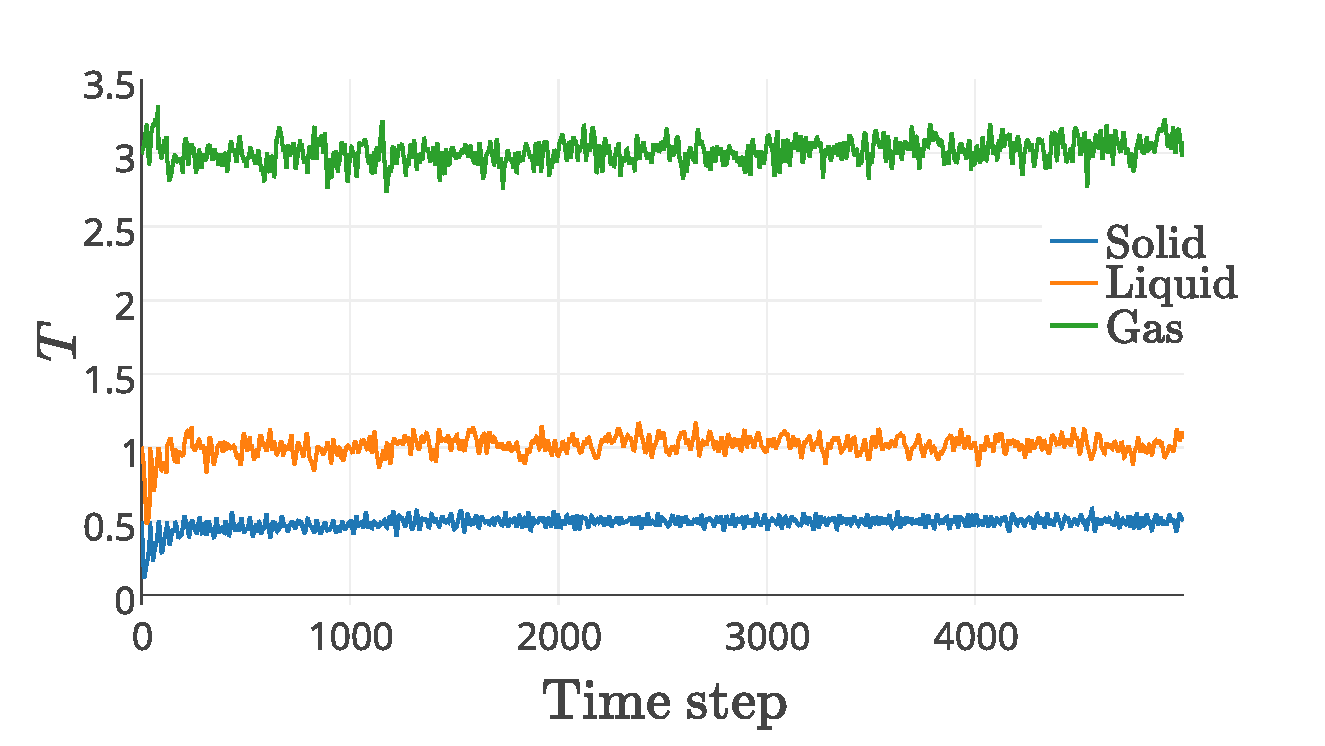
\includegraphics[scale=0.4]{instanteneous_temperature.eps}
 \captionof{figure}{Instantaneous temperatures for different phases of argon. Gas had $\rho = 0.3$,$T_d = 3$, liquid had $\rho = 0.8$,$T_d = 1$ and solid had $\rho = 1.2$, $T_d = 0.5$ as parameters. Note the increase in fluctuations for higher temperatures.}\label{fig:Inst_temp}
\end{Figure}

\begin{Figure}
  \centerfloat
     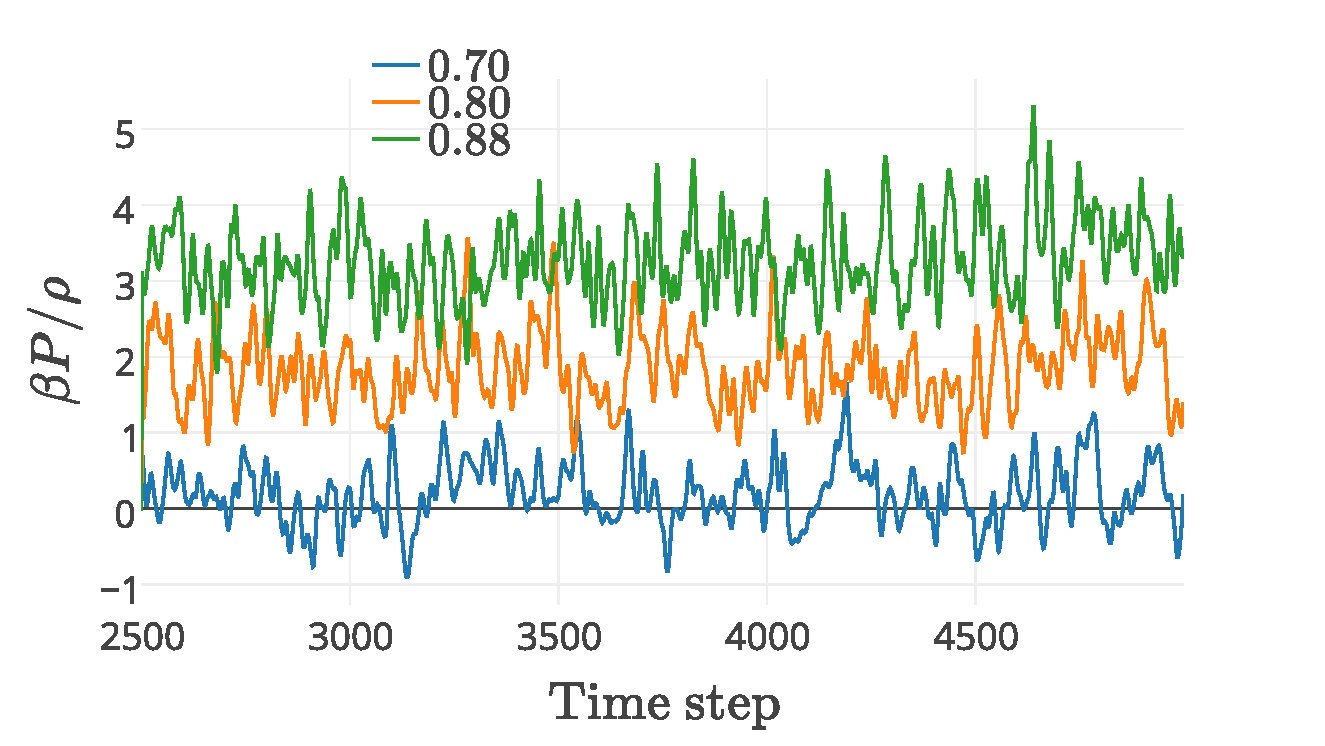
\includegraphics[scale=0.4]{instanteneous_pressure.eps}
 \captionof{figure}{Instantaneous pressure for several different values of $\rho$ at $T = 1$ in the argon liquid phase.}\label{fig:Inst_pressure}
\end{Figure}

\begin{Figure}
  \centerfloat
     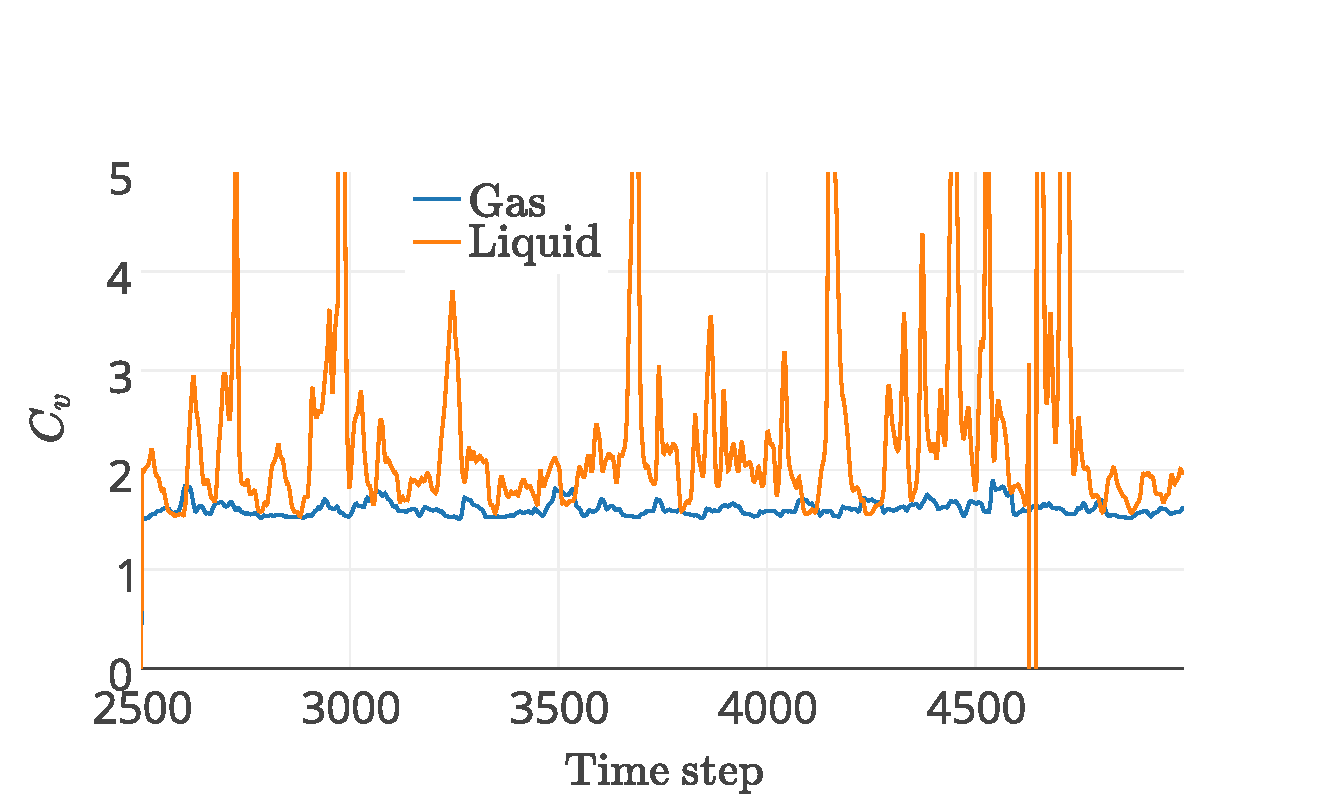
\includegraphics[scale=0.4]{specific_heat.eps}
 \captionof{figure}{Comparison between the instantaneous specific heat for gaseous $(\rho = 0.3$,$T_d = 3)$ and liquid ($\rho = 0.8$,$T_d = 1$) argon. }\label{fig:specific_heat}
\end{Figure}


\begin{Figure}
  \centerfloat
     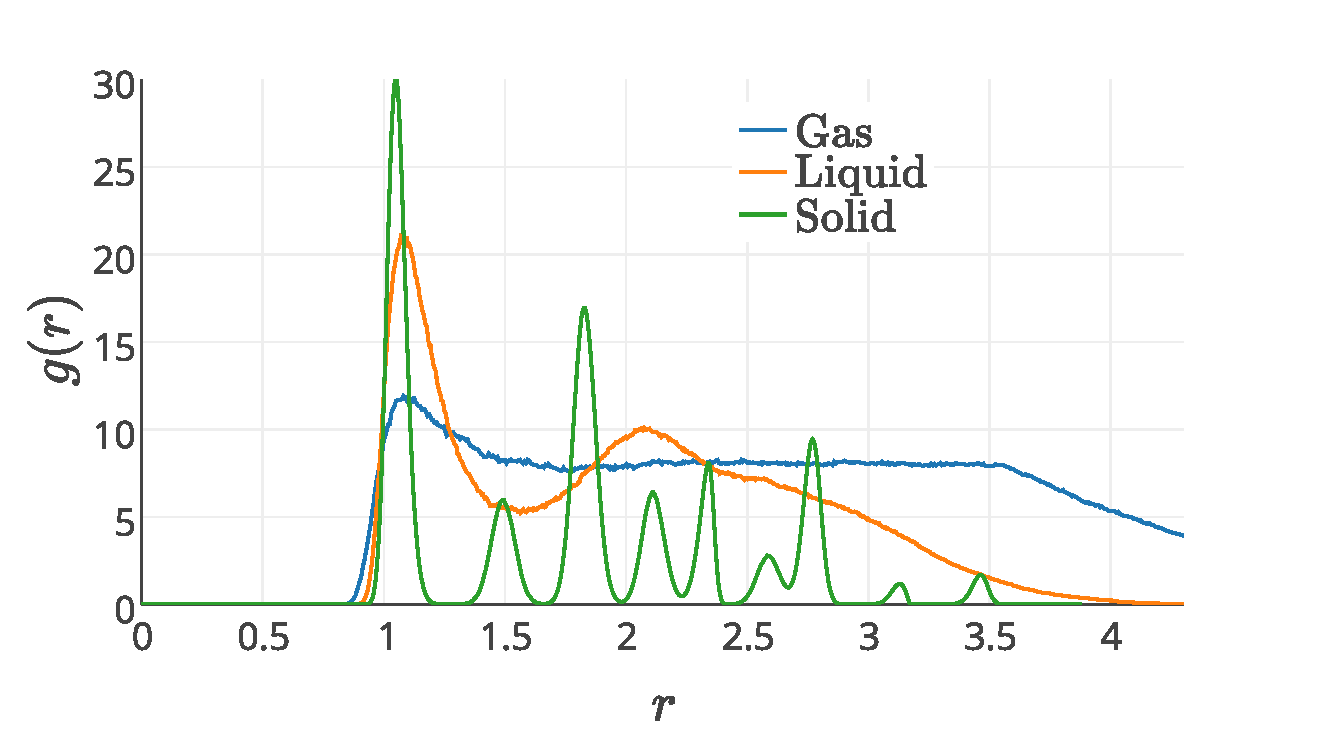
\includegraphics[scale=0.4]{correlation_function.eps}
 \captionof{figure}{Comparison of the (unnormalized) correlation function for different phases of argon. Gas had $\rho = 0.3$,$T_d = 3$, liquid had $\rho = 0.8$,$T_d = 1$ and solid had $\rho = 1.2$, $T_d = 0.5$ as parameters.}\label{fig:Correlationfunctions1}
\end{Figure}
